% This must be in the first 5 lines to tell arXiv to use pdfLaTeX, which is strongly recommended.
\pdfoutput=1
% In particular, the hyperref package requires pdfLaTeX in order to break URLs across lines.

\documentclass[11pt]{article}

% Change "review" to "final" to generate the final (sometimes called camera-ready) version.
% Change to "preprint" to generate a non-anonymous version with page numbers.
\usepackage[preprint]{acl}
% Standard package includes
\usepackage{times}
\usepackage{latexsym}
\usepackage{multirow}
\usepackage{booktabs}
\usepackage{subfigure}
\usepackage{tcolorbox}
\usepackage{amsmath}

% For proper rendering and hyphenation of words containing Latin characters (including in bib files)
\usepackage[T1]{fontenc}
\usepackage[T2A]{fontenc} 
% For Vietnamese characters
% \usepackage[T5]{fontenc}
% See https://www.latex-project.org/help/documentation/encguide.pdf for other character sets

% This assumes your files are encoded as UTF8
\usepackage[utf8]{inputenc}

% Russian language
\usepackage[russian]{babel}

% This is not strictly necessary, and may be commented out,
% but it will improve the layout of the manuscript,
% and will typically save some space.
\usepackage{microtype}

% This is also not strictly necessary, and may be commented out.
% However, it will improve the aesthetics of text in
% the typewriter font.
\usepackage{inconsolata}

%Including images in your LaTeX document requires adding
%additional package(s)
\usepackage{graphicx}

% If the title and author information does not fit in the area allocated, uncomment the following
%
%\setlength\titlebox{<dim>}
%
% and set <dim> to something 5cm or larger.

\title{Применение синтетических данных, полученных с помощью генеративной нейросети, для повышения качества моделей детекции.}

% Author information can be set in various styles:
% For several authors from the same institution:
% \author{Author 1 \and ... \and Author n \\
%         Address line \\ ... \\ Address line}
% if the names do not fit well on one line use
%         Author 1 \\ {\bf Author 2} \\ ... \\ {\bf Author n} \\
% For authors from different institutions:
% \author{Author 1 \\ Address line \\  ... \\ Address line
%         \And  ... \And
%         Author n \\ Address line \\ ... \\ Address line}
% To start a separate ``row'' of authors use \AND, as in
% \author{Author 1 \\ Address line \\  ... \\ Address line
%         \AND
%         Author 2 \\ Address line \\ ... \\ Address line \And
%         Author 3 \\ Address line \\ ... \\ Address line}

\author{
    \textbf{Andrei Filatov\thanks{\quad These authors contributed equally to this work.}\textsuperscript{1, 3}},
    \textbf{Daniil Dorin\footnotemark[1]\textsuperscript{2}},
    \textbf{Nikita Barinov\textsuperscript{2, 3}},
    \textbf{Uliana Izmesteva\textsuperscript{2}}, 
\\
    \textbf{Igor Ignashin\textsuperscript{2}},
    \textbf{Ilya Stepanov\textsuperscript{2}}, 
    \textbf{Viacheslav Vasilev\textsuperscript{2, 3}},
    \textbf{Maxim Kurkin\textsuperscript{1, 3}}, 
\\
    \textbf{Dmitry Yudin\textsuperscript{2,3}},
    \textbf{Aibek Alanov\textsuperscript{3, 5}},
    \textbf{Sergey Zagoruyko\textsuperscript{1, 4}},
\\ 
    \textbf{Denis Dimitrov\textsuperscript{3}},
    \textbf{Andrey Kuznetsov\textsuperscript{3}}
\\
\\
    \textsuperscript{1}Center for Artificial Intelligence Technology,
    \textsuperscript{2}MIPT,
    \textsuperscript{3}AIRI,
    \textsuperscript{4}MTS AI,
    \textsuperscript{5}HSE University
\\
     \small{
       \textbf{Correspondence:} \href{mailto:filatovandreiv@gmail.com}{filatovandreiv@gmail.com}
    }  
}

% Andrei Filatov, Daniil Dorin, Uliana Zemtsova, Igor Ignashin, Ilya Stepanov, Nikita Barinov, Dmitry Udin, Aibek Alanov, Andrey Kuznetsov, Denis Dimitrov, Sergey Zagoryuko, Viacheslav Vasilev, Maxim Kurkin.

%\author{
%  \textbf{First Author\textsuperscript{1}},
%  \textbf{Second Author\textsuperscript{1,2}},
%  \textbf{Third T. Author\textsuperscript{1}},
%  \textbf{Fourth Author\textsuperscript{1}},
%\\
%  \textbf{Fifth Author\textsuperscript{1,2}},
%  \textbf{Sixth Author\textsuperscript{1}},
%  \textbf{Seventh Author\textsuperscript{1}},
%  \textbf{Eighth Author \textsuperscript{1,2,3,4}},
%\\
%  \textbf{Ninth Author\textsuperscript{1}},
%  \textbf{Tenth Author\textsuperscript{1}},
%  \textbf{Eleventh E. Author\textsuperscript{1,2,3,4,5}},
%  \textbf{Twelfth Author\textsuperscript{1}},
%\\
%  \textbf{Thirteenth Author\textsuperscript{3}},
%  \textbf{Fourteenth F. Author\textsuperscript{2,4}},
%  \textbf{Fifteenth Author\textsuperscript{1}},
%  \textbf{Sixteenth Author\textsuperscript{1}},
%\\
%  \textbf{Seventeenth S. Author\textsuperscript{4,5}},
%  \textbf{Eighteenth Author\textsuperscript{3,4}},
%  \textbf{Nineteenth N. Author\textsuperscript{2,5}},
%  \textbf{Twentieth Author\textsuperscript{1}}
%\\
%\\
%  \textsuperscript{1}Skoltech 1,
%  \textsuperscript{2}MIPT 2,
%  \textsuperscript{3}Sber AI 3,
%  \textsuperscript{4}AIRI 4,
%  \textsuperscript{5}MTS AI 5
% \\
%  \small{
%    \textbf{Correspondence:} \href{mailto:email@domain}{email@domain}
%  }
%}

% What problem does the proposed system address? Проблема того, что создание данных для сегментации/детекции достаточно сложно требовательная процедура в плане разметчиков, поэтому достаточно сложно получить большой датасет, который покрывает все случаи. Также датасеты ограниченны в одном наборе и объектов и разметок, что не позволяет их использовать на новых данных. Например, если в датасете COCO большинство фенов расположены на стенах.

% Why is the system important and what is its impact? Наша система позволит аугментировать текущие датасеты таких образом улучшить качество детекции на текущих данных, а также расширить текущие датасеты по детекции на новые объекты, классы, которых раньше не было в выборке. Таким образом, наша система значимо расширяет возможности 
% What is the novelty in the approach/technology on which this system is based? Новизна данной системы в том, что мы первые предлагаем подход по аугментации данных за счёт добавлениях новых классов аннотации и изменения аннотации в исходных данных. Таким образом, данных подход позволяет значимо расширить возможности детекции, так как новые классы можно будет добавить в любой датасет и так же сделает модель более устойчивой. 
% Who is the target audience? Любой специалист, который работает с детекционными сегментационными данными
% How does the system work? Система работает в двух режимах: интерактивном и автоматическом 
% How does it compare with existing systems? For our best knowledge, не существует системы, которая выполняет полностью автоматическую замену классов аннотаций. Из конкурентов существуют только copy paste augmentation, но они могут быть semantically harmful, а также системы по аугментации текущих классов аннотаций при этом они ни как не меняют класс аннотации. Таким образом, наш подход ортогонален текущим работам и с легкостью может быть дополнен их результатами.
% How is the system licensed? Apache licence.
% How was the system evaluated? Were user studies/human evaluation experiments conducted?
% Для проверки системы мы провели её оценку на датасетах по детекции и сегментации, чтобы проверить эappenективность её качества. Можно провести user studies, чтобы проверить насколько люди смогли отличить аугментированные изображения.

% Рассказать про задачу, почему она важна? Какую проблемную зону решает? Текущие методы семантически не обогощают выборку по средством изменения. Изображение. Что мы предлагаем шаг за шагом? Мы предлагаем это делать таким образом и даёт такие бенефиты? В части метод описать метод? Описать эксперименты? Мы рассматриваем такой сетап, который работает? Последовательно и ясно и нейтрально и приятно читать?

\begin{document}
\twocolumn[{%
\renewcommand\twocolumn[1][]{#1}%
\maketitle
\begin{center}
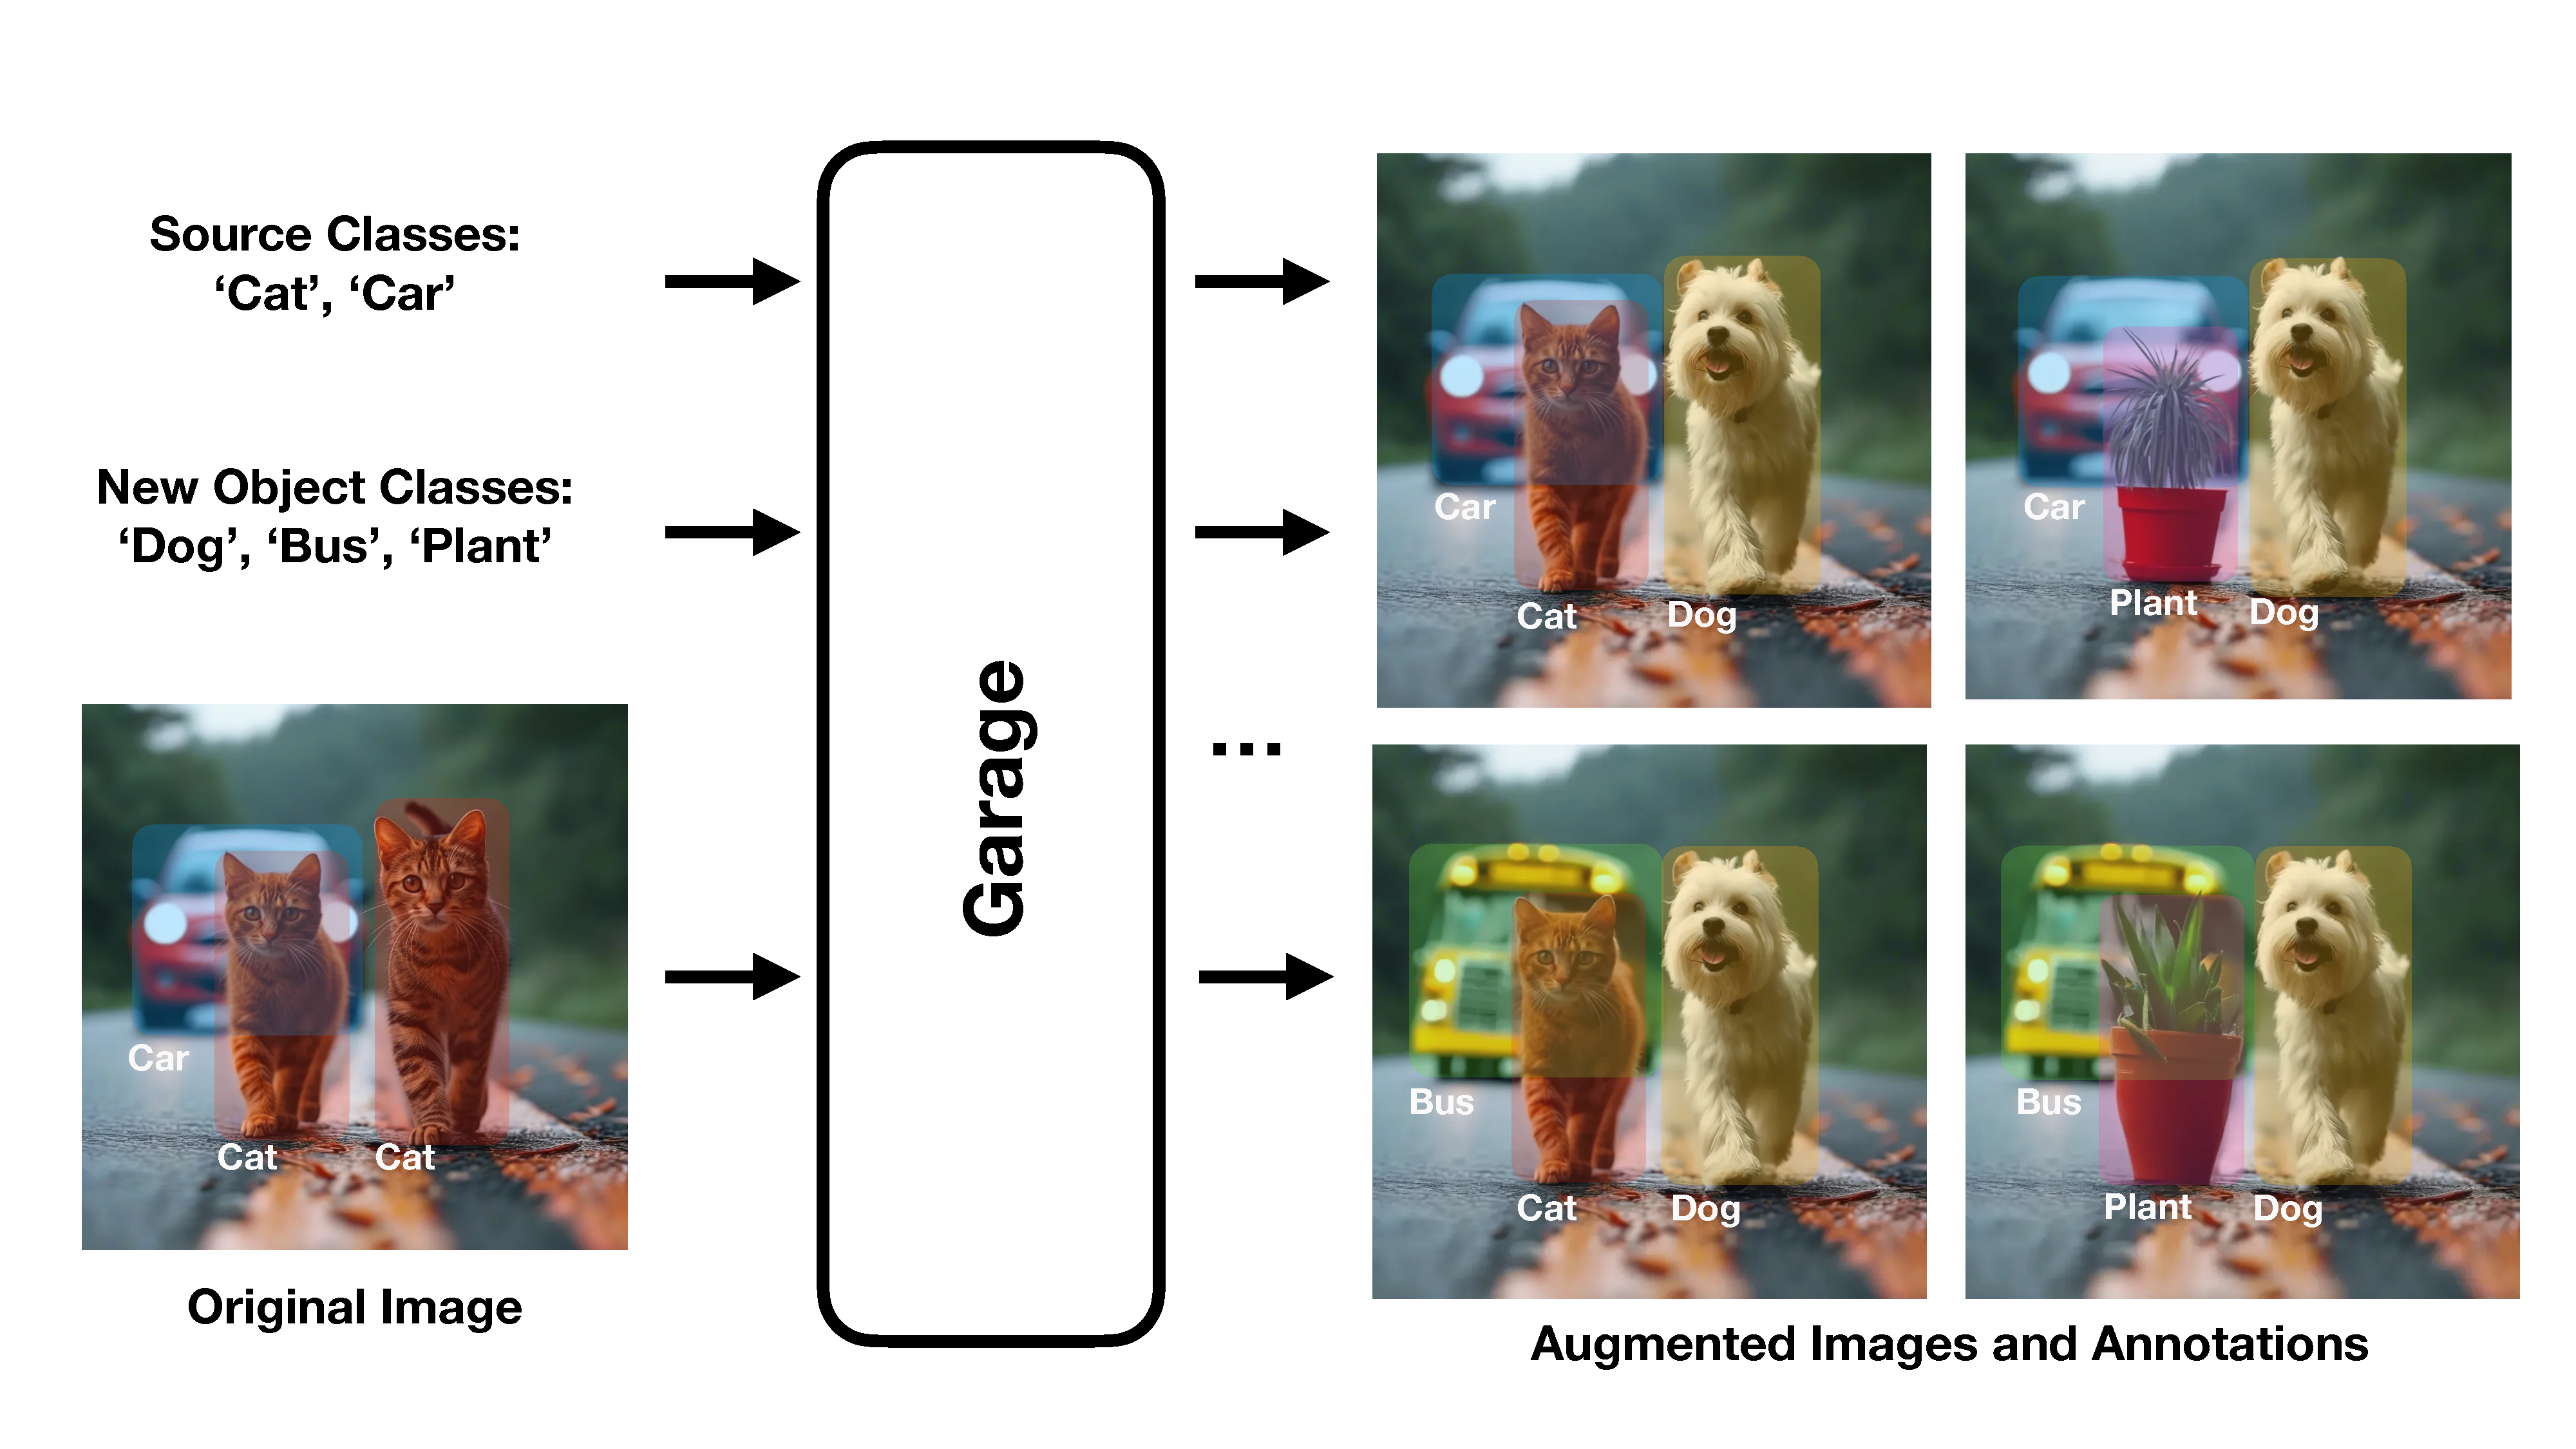
\includegraphics[width=\textwidth]{figures/Graphical Abstract - GARAGE.pdf} % Adjust the path and width as necessary
\captionof{figure}{Исходное изображение (слева) изображает двух кошек, идущих по дороге, с машиной на заднем плане. Вариации включают замену кошки на растение, кошки на собаку и машины на автобус. Данные аугментации показывают, как генеративные модели могут создавать разнообразные примеры для обучения, изменяя различные элементы исходного изображения, что способствует повышению устойчивости моделей компьютерного зрения.} % Added caption
\end{center}
}]

% Языковые модели при этом обладают большим знанием о мире, его устройстве и семантике и если передать это знание в датасет, то можно было бы значительно обогатить visual разнообразие данных и улучшить качество визуальных моделей

% С помощью VLM мы получаем описание изображение, далее с помощью языковые моделей мы определяем, что можно заменить на изображении и составляем расширенный промпт, по которому генерируется модификация данных, таким образом мы семантически значимо аугментируем датасет.

\begin{abstract}
Аугментация данных играет ключевую роль в улучшении производительности моделей машинного обучения, особенно в области компьютерного зрения. Традиционные методы, такие как повороты, сдвиги и регулировка яркости, ограничены в своей способности обеспечивать значительные семантические вариации, что часто приводит к плохому обобщению на новые данные.

В данной статье мы представляем новый подход, который позволяет заменять объекты на изображениях. Используя Visual-Language Models, мы получаем описания изображений, а затем, используя языковые нейросети, определяем, что можно заменить на изображении и составляем расширенный запрос, с помощью которого можем генерировать модифицированные данные. Таким образом, мы увеличиваем количество данных с использованием осмысленных запросов.

Мы демонстрируем эффективность данного подхода, проводя бенчмаркинг моделей, обученных с аугментированными и без аугментированных данных, показывая улучшения в производительности моделей детекции.


% Для детекции и сегментации требуется очень много усилий, чтобы получить разметку данных из-за чего датасеты получаеются достаточно маленькими. В этой работе мы предлагаем наш инструмент Garage, интерактивный и при этом полностью автоматический пайлайн по созданию семантически обоснованных сегментаций данных. С помощью этого инструмента можно расширить уже известные датасеты обогатив их новыми классами или добавить разнообразия к текущем датасетам. 

\end{abstract}

\section{Введение}
% Глобально хочется рассказать о том, что была проблема в том, в компьютерном зрении всегда стояла проблема необходимости создания качественных данных. Особенно остро этот вопрос стоит в сегментации и детекции, где на разметку одного изображения уходит до нескольких минут разметчкика. Традиционным подходом по увеличению числа качественных данных являются аугментация, они позволяют значимо расширить датасет для обучения. Однако, данных подходы ограничены цветовыми преобразованиями, фокусом на отдельные регионы при аугментации. Также они жестко ограничены тем, чтобы была возможность аугментировать данные семантически значимо. То есть на том же изображении мы не можем увидеть другие объекты, которых не было на изображении, например увидеть Капибару в датасете COCO.

% Чтобы адресовать эту проблему мы презентуем нашу фреймворк Garage. Это фреймворк позволяет семантически аугментировать изображения, добавляя  \textit{\textit{}}

% \begin{figure*}
%     \centering
%     % https://drive.google.com/file/d/1PAz5huRwpn1Ble3HGoWgeP2Z8_EThgjl/view?usp=drive_link
%     \includegraphics[width=1\textwidth]{figures/demo_scheme_final.png}
%     \caption{\textbf{Demo}. Данная Demo проста в использовании и предоставляет пользователям опции для выбора объектов и вариантов дополнений, что позволяет легко генерировать аугментированные изображения. Процесс начинается с загрузки изображения с вашего компьютера или выбора из предоставленных примеров. После загрузки изображения пользователь может настроить объект для сегментации. Это можно сделать либо через текстовый запрос в модели GroundedSAM, либо выбрав маску из предложенных примеров. Наконец, пользователь настраивает целевой объект для дополнения. Инструмент сгенерирует изображение c целевым объектом.}
%     \label{fig:demo}
% \end{figure*}

Аугментация данных — важный инструмент в арсенале современных исследователей в области машинного обучения и компьютерного зрения. Она позволяет увеличить объём данных, улучшая общую производительность моделей путём создания различных вариаций. Однако традиционные методы аугментации, такие как повороты, сдвиги и изменения яркости, ограничены в своих возможностях. Они не обеспечивают значительных семантических расширений данных, что могло бы существенно улучшить обучение моделей. Например, при обучении модели детекции стандартные методы аугментации, такие как повороты и масштабирование, не создают достаточного разнообразия объектов на изображениях. Это может привести к тому, что модели не будут хорошо обобщаться на новые данные.

% Один из возможных способов решить эту проблему использование генеративных моделей. Генеративные модели позволяют создать новые аугментации, либо по средством генерирования новых изображений, либо по аугментации текущих изображений. Однако, недостаток первого подхода в том, что генерация полной картинок слишком отличается от распределения исходного датасета, а модели, которые аугментирует текущее изображения только меняет исходное layout изображения, тем самым не позволяя добавить новый класс в датасет.


% ) упомянуть в интро другие генеративные аугментации и почему их пока недостаточно (видел, что ты их упоминаешь в релейтед ворк, но в интро тоже нужно об этом сказать)

В этой работе мы предлагаем новую модель для аугментации данных, которая позволяет заменять объекты на изображениях. Этот подход семантически увеличивает объем данных, что важно для улучшения способности моделей машинного обучения к обобщению.

% Мы разработали систему, которая работает в двух режимах: интерактивном и автоматическом. В интерактивном режиме пользователь может вручную выбрать объект для дополнения и указать объект, который его заменит. Это позволяет более точно контролировать процесс аугментации и адаптировать его под конкретные потребности. В автоматическом режиме система автоматически выбирает объекты на изображении и заменяет их объектами из заданных пользователем классов. Это позволяет быстро генерировать большие объемы данных с разнообразными семантическими сочетаниями.

Наши вклады следующие:
\begin{itemize}
    \item Мы представляем модель для аугментации данных, предназначенную для замены объектов, что обеспечивает значительное семантическое обогащение наборов данных.
    \item Мы демонстрируем экспериментальные результаты, которые показывают улучшенные способности к обобщению моделей, обученных на наших дополненных данных.
    % доступна\footnote{\href{https://youtu.be/QUpuwwhd3qw}{Видео-демонстрация}}.
    \item Мы предлагаем открытое исходное решение, позволяя исследовательскому сообществу воспользоваться нашими достижениями в области аугментации данных. 
    % \Код опубликован на GitHub.\footnote{\href{https://github.com/DorinDaniil/Garage}{Github repository}}
\end{itemize}

\section{Архитектура(Приложение?)}

\begin{figure*}[h]
    \centering
    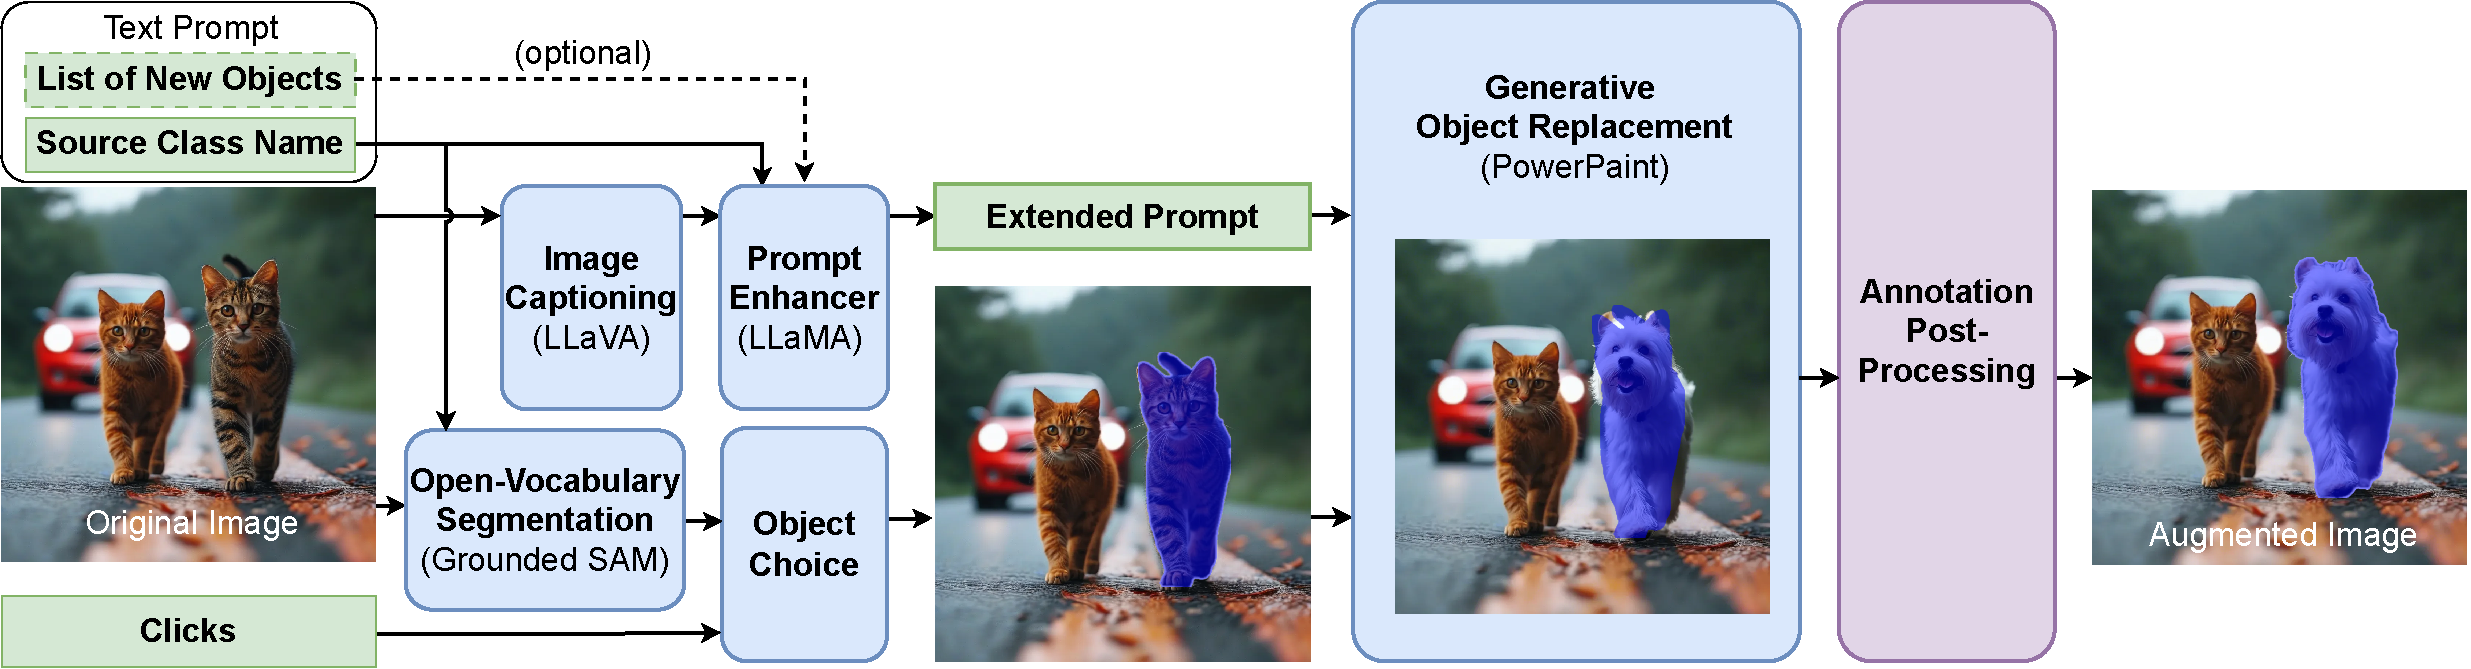
\includegraphics[width=\textwidth]{figures/scheme_augmented.pdf}
    \caption \textbf{Детали архитектуры}. На рисунке показаны последовательные этапы работы системы. Он включает в себя:
\textbf{Выбор объекта:} Выбор объекта на основе пользовательских запросов.
\textbf{Аугментация:} Генерация аугментации с дополнительными пользовательскими запросами или автоматическим выбором.
\textbf{Постобработка:} Удаление артефактов генерации и фильтрация некорректных примеров. Каждый этап важен для получения качественных результатов.
    \label{fig:internal_framework}
\end{figure*}

% Наш фреймворк позволяет работу в двух режимах автоматическом и ручной режим

\subsection{Интерактивная аугментация}

Рабочий процесс интерактивной аугментации следующий:

\begin{itemize}
    \item Пользователь загружает изображение и выбирает объект для замены, используя текстовый запрос для описания объекта, который передается в модель GroundedSAM \cite{ren2024grounded} для извлечения маски объекта.
    \item Пользователь указывает класс, на который будет заменен исходный объект.
    \item Наша модель расширяет предоставленный запрос с помощью LLaMA \cite{dubey2024llama} и генерирует дополненное изображение с замененным объектом с использованием PowerPaint \cite{zhuang2023task}.
\end{itemize}

\subsection{Автоматическая аугментация}

Помимо ручной аугментации, наша система предлагает полностью автоматический режим.

После загрузки исходного набора данных пользователи могут указать, какие классы нужно добавить или дополнить. Например, если пользователь хочет добавить класс "капибара", он может указать это, и класс будет включен в набор данных. Затем система автоматически генерирует необходимые аугментации, в результате чего набор данных расширяется. Эта комплексная система состоит из трех этапов, описанных ниже.

\subsection{Выбор объекта}

Первый этап заключается в выборе объекта для аугментации. Для автоматического выбора мы используем LLaVA \cite{liu2024llavanext} для идентификации объектов, которые могут быть заменены, и предоставления описания изображения. LLaVA извлекает список объектов с изображения, из которого случайным образом выбирается объект для аугментации. Затем мы применяем GroundedSAM \cite{kirillov2023segment} для генерации маски объекта на основе выбранного объекта. Для подробностей о запросах LLaVA, пожалуйста, смотрите Приложение \ref{sec:appendix}.

\subsection{Аугментация}

Когда объект для аугментации выбран, используется LLaMA \cite{dubey2024llama} для генерации подходящей замены. Пользователь может предоставить список потенциальных объектов для замены, из которого модель сделает окончательный выбор. Если список не предоставлен, объект будет выбран автоматически. Кроме того, модель получает полное описание изображения от LLaVA, чтобы гарантировать, что LLaMA полностью понимает контекст.

Для генерации замены мы применяем технологию встраивания объектов PowerPaint \cite{zhuang2023task} с выбранным запросом. В ходе исследования мы выявили проблему: создание объекта с коротким запросом обычно дает неудовлетворительные результаты. Поэтому мы расширяем запрос с использованием LLaMA для предоставленного запроса. В конце процедуры расширенный запрос передается в PowerPaint для получения аугментированного изображения.

\subsection{Последующая обработка}

Мы применяем двухэтапную постобработку. На первом этапе мы используем Alpha-CLIP \cite{sun2024alpha} для фильтрации некачественной генерации. Alpha-CLIP действует как обычный CLIP \cite{Radford2021}, но принимает маску, что позволяет вычислять сходство с конкретной областью изображения. Если значение CLIP превышает определенный порог, мы принимаем сгенерированную аугментацию. В противном случае мы генерируем изображение заново. После того как изображение прошло оценку CLIP, мы применяем SAM для получения более качественной генерации объекта. Это необходимо, потому что встраивание часто генерирует новый объект, не совсем точно соответствующий аннотации, поэтому нужно применить коррекцию для получения правильной маски. Несоответствие между объектом и маской можно увидеть на Рисунке \ref{fig:internal_framework}.

\section{Эксперименты}

% Больше деталей на эксперимент

Для проверки эффективности нашего подхода к аугментации мы провели эксперименты с аугментациями на наборе данных VOC~\cite{everingham2010pascal}.

\subsection{Добавление нового класса}

% 
Один из возможных вариантов применения нашего метода -- генерация данных для класса, который отсутствует или представлен ограниченно в существующем наборе данных.

Для проверки данного применения мы провели следующий эксперимент. Из набора данных VOC мы удалили данные c определённым классом, например, классом "кошка". Затем мы выполнили аугментацию данных на оставшихся данных, чтобы добавить отсутствующий класс в выборку. Во время процесса аугментации предложенный алгоритм применялся ко всем изображениям в наборе данных, на которых не был представлен этот класс.


(Вот тут вообще не понял что имелось ввиду)
Для изображений с несколькими объектами случайным образом выбирался один, чей Bounding Boxes находился в пределах относительной площади не более 0.5, если такие объекты были доступны. Это было сделано для того, чтобы избежать наложения маленьких объектов в процессе генерации.

Затем мы обучили модели детекции (FasterRCNN \cite{ren2015faster}, DETR \cite{carion2020end}, YOLOv10-N \cite{jocher2023yolo}) на данных с различными аугментациями отсутствующего класса, чтобы исследовать влияние наших аугментированных данных на результаты. Для обучения мы использовали стандартные скрипты из MMDetection \cite{chen2019mmdetection} и Ultralytics \cite{jocher2023yolo}. Результаты представлены в таблице \ref{tab:combined-results}. Из наших экспериментов видно, что использование нашего метода улучшает качество детекции отсутствующего класса при сохранении общего качества модели на том же уровне. Важно отметить, что качество детекции для других классов не изменилось.

% One of possible application of our framework is generating data for an absent class in existing dataset. 
% Почему? Добавление аугментации определенного объетка может помочь в случае объект определенного класса отсутствует в данных, то добавить его. А в случае его присутствия сделать выборку данных более разнообразными. Для проверки этого применения мы провели следующий эксперимент. Из данных датасетов COCO и color мы выкинули данные определенного класса: для VOC это potted plant (как класс с самым худшим качеством) и класс cat. Для COCO это class <> and <>. Затем мы запустили аугментацию данных на оставшихся данных таким образом, чтобы добавить отсутствующий класс в выборку. При аугментации <>

% Далее, мы поставили обучаться модели детекции FasterRCNN, DETR,   YOLOv10-N-N на данных с различным добавлением отсутствующего класса, чтобы проверить насколько сильно влияние наших аугментированных данных на полученный результат. The result are presented in the Table. \ref{tab:voc-results}.  By results of our experiments we see that usage of our framework improves quality of cat detection whilst keeping the overall quality of the model on the same level. Важно отметить, что качество детекции на других классах не изменилось.

\begin{table*}[]
\centering
\caption{Результаты детекции объектов на наборе данных Pascal VOC. Результаты показывают, что обучение на наших данных значительно улучшает производительность модели при различных процентах данных, что подтверждается более высокими значениями mAP в строках "наши" по сравнению с "оригинальные". Проценты представляют собой долю изображений с кошками, использованных из оригинального набора данных.:}
\begin{tabular}{ccc|ccccc}
\toprule
\textbf{Датасет} & \textbf{Модель} & \textbf{Данные} & \textbf{0\%} & \textbf{25\%} & \textbf{50\%} & \textbf{75\%} & \textbf{100\%} \\ 
\midrule
\multirow{6}{*}{\textbf{Pascal VOC}} & \multirow{2}{*}{\textbf{DETR}} & оригинальные & 0.0 & \textbf{57.5} & 61.5 & 65.4 & 69.1 \\ %\cline{3-8} 
 & & наши & \textbf{5.3} & 55.6 & \textbf{62.2} & \textbf{66.3} & \textbf{70.3}

 \\ 
\cline{2-8}
 & \multirow{2}{*}{\textbf{ YOLOv10-N}} & оригинальные & 0.0 & 50.9 & \textbf{54.8} & 56.9 & 60.4 \\ %\cline{3-8} 
 & & наши & \textbf{31.5} & \textbf{51.3} & 53.6 & \textbf{57.9} & \textbf{61.3} \\ 
\cline{2-8}
 & \multirow{2}{*}{\textbf{Faster RCNN}} & оригинальные & 0.0 & 74.5 & 77.4 & 75.5 & 76.6 \\ %\cline{3-8} 
 & & наши & \textbf{66.4} & \textbf{77.3} & \textbf{80.1} & \textbf{83.5} & \textbf{84.0} \\ 
% \midrule
% \multirow{6}{*}{\textbf{COCO}} & \multirow{2}{*}{\textbf{DETR}} & original & & & & & \\ \cline{3-8} 
%  & & ours & & & & & \\ 
% \cline{2-8}
%  & \multirow{2}{*}{\textbf{ YOLOv10-N}} & original & & & & & \\ \cline{3-8} 
%  & & ours & & & & & \\ 
% \cline{2-8}
%  & \multirow{2}{*}{\textbf{Faster RCNN}} & original & - & - & - & - & - \\ \cline{3-8} 
%  & & ours & & & & & \\ 
\bottomrule
\end{tabular}
\label{tab:combined-results}
\end{table*}

% \subsection{Standard augmentation}

% % To check applicability of our framework as a general tool for augmentations. We conducted experiments to compare our augmentation with augmentation with other frameworks.
% % Вторым экспериментом мы проверили, насколько эффективно использование нашего фреймворка как общего инструмента по аугментации данных. Для мы решили провести эксперименты на VOC/COCO датасете. Для этого мы засэмплировали часть общей выборки в 25%/50%/75%/100% и примененили наши аугментации. Аугментировали мы данные по следующей процедуре <>
% % Результаты представлены в таблицах \ref{tab}. По результатам можно отметить, что модель стабильно добавляет качество в экспериментах.

% To check the applicability of our framework as a general tool for augmentations, we conducted experiments to compare our augmentation with augmentations from other frameworks.

% In the second experiment, we evaluated the effectiveness of our framework as a general tool for data augmentation. We decided to conduct experiments on the VOC/COCO dataset. We sampled a portion of the total dataset at 25\%, 50\%, 75\%, and 100\%, and applied our augmentations. The data were augmented according to the following procedure: <>

% The results are presented in Table \ref{tab:general-coco-results} and Table \ref{tab:general-voc-results}. From the results, it can be noted that our model consistently improves quality across the experiments.



\subsection{Улучшение качества подсказок}
При использовании стандартных подсказок мы заметили снижение визуального качества генерируемых изображений, особенно при более коротких подсказках, таких как простые метки классов. Чтобы решить эту проблему, мы использовали расширенные подсказки, воспользовавшись лингвистическими возможностями модели LLaMA. Например, простая инструкция, такая как \emph{cat} (кошка), может быть расширена в более описательную фразу, например, \emph{The ginger tabby cat has a sleek body, pointy ears, and curious green eyes gazing around from its playful pose} (Имбирная полосатая кошка с изящным телом, острыми ушами и любопытными зелёными глазами, оглядывающимися вокруг с игривой позы). Это расширение вводит важную контекстную информацию, эффективно сокращая разрыв между текстовыми и визуальными представлениями.

Чтобы оценить важность расширения подсказок при обучении модели, мы провели эксперимент, создав два набора данных с идентичными изображениями: один с использованием только базовой подсказки, а другой — с расширенной подсказкой, включающей текстовое описание изображения. Этот подход позволил нам оценить, как расширенные подсказки могут улучшить качество генерируемых изображений. Расширенные инструкции предоставили последующей модели PowerPaint подробную информацию и нюансы, что позволило создавать изображения более высокого качества, разнообразные и визуально последовательные, соответствующие инструкции.

Как уже упоминалось, генерация объекта с использованием короткой инструкции обычно приводит к низкому качеству. Мы провели дополнительный эксперимент, чтобы изучить, как расширение подсказки влияет на обучение модели детекции объектов. Мы обучили модель FasterRCNN на наборе данных, где не было изображений кошек, используя классическую подсказку и расширенную подсказку. Результаты показаны в таблице \ref{fig:expanding_prompts}. Из результатов видно, что расширенная подсказка улучшает качество аугментированных данных и, следовательно, модель детекции.

\begin{figure}[h]
    \centering
    \includegraphics[width=0.47\textwidth]{figures/ablation_llama_new.pdf}
    \caption{\textbf{Сравнение генерации в зависимости от расширения подсказки.} Изображения слева, сгенерированные с использованием расширенных подсказок, демонстрируют значительно большее количество деталей и точности по сравнению с изображениями справа, сгенерированными с минимальными подсказками. Это показывает, как наша модель работает лучше с подробными описаниями, более эффективно захватывая нюансы и особенности желаемого результата.}
    \label{fig:expanding_prompts}
\end{figure}

\begin{table}[h]
        \centering
        \begin{tabular}{cc}
                \toprule
                \multicolumn{2}{c}{\textbf{AP on \emph{cat} category}} \\
                % \midrule
                w/o expanded prompts & expanded prompts   \\
                \midrule
                % \hline
                  64.6  &  \textbf{66.4} \\ %\hline
                  \bottomrule
        \end{tabular}
        \caption{\textbf{Сравнение качества обучения модели FasterRCNN в зависимости от расширения инструкции.} Расширение подсказки улучшает качество модели. Результаты показывают, что использование расширенных подсказок значительно повышает среднюю точность (AP) для категории "кошка" по сравнению с использованием подсказок без расширения.}
        \label{tab:prompt_expanding}
        
\end{table}

% \subsection{Augmentation of segmentation datasets}
% \textcolor{red}{The proposed method is not limited to detection masks, it is possible to argue for the segmentation mask of the object in the figure ..need images examples are given.}

\section{Смежные работы}

Аугментация данных -- это широко используемая техника в области машинного обучения и компьютерного зрения для увеличения разнообразия и объема обучающих наборов данных. Традиционные методы аугментации данных, такие как повороты, обрезка и изменение яркости цветов, стали основой для повышения устойчивости моделей \cite{buslaev2020albumentations}. Например, \cite{krizhevsky2012imagenet} продемонстрировал эффективность этих техник в своей работе по задаче классификации на наборе данных ImageNet. Однако эти методы часто не способны повысить качество сложных моделей.

Более современные подходы используют генеративные модели в качестве источников для создания аугментаций. \cite{alimisis2024advances} исследует использование передовых генеративных моделей для создания разнообразных и реалистичных аугментаций. \cite{yin2023ttida} использовали модели "text-to-text" и "text-to-image" для генерации аугментаций для задач классификации изображений, продемонстрировав значительные улучшения в производительности модели. \cite{fang2024data} использовали адаптер ControlNet для генерации аугментаций, что повысило вариативность и устойчивость набора данных. \cite{kupyn2024dataset} применили методы InPaint для аугментации данных, сохраняя при этом те же аннотации меток.

Альтернативой аугментациям, которые улучшают семантику, является Open Vocabulary Detection \cite{wu2024towards}, где модель учится обнаруживать объекты с использованием языковой модели. Хотя этот подход эффективен, он ограничен словарем объектов, на котором модель была обучена, и не позволяет увеличивать разнообразие набора данных через уточнение свойств обнаруживаемых объектов. Более того, создание таких архитектур требует значительных ресурсов, что может стать существенным ограничением при обучении эффективной модели.


(Вот тут ощущение, что вода, не очень понимаю почему остальные модели улучашют существующие а наша типо генерит новые)
Наша работа отличается от предыдущих подходов к генеративной аугментации тем, что она позволяет не просто улучшать существующие, а семантически и структурно дополнять набор данных, предлагая более комплексную стратегию аугментации.

\section{Вывод / Ограничения}

В данной статье мы представили новый подход, предназначенный для решения задач, связанных с аугментацией данных в машинном обучении и компьютерном зрении.

Мы продемонстрировали эффективность нашей нейросети через всесторонние эксперименты и бенчмаркинг. Результаты показали, что модели, обученные на данных, аугментированных с помощью нашего подхода, демонстрируют улучшения. 

% Расширяемая архитектура \textbf{Garage} позволяет легко интегрировать новые методы аугментации и настраивать платформу в соответствии с конкретными потребностями. Эта гибкость гарантирует, что наша платформа может адаптироваться к различным типам данных и областям, предлагая надежное решение для аугментации обучающих наборов данных.

Одним из ограничений нашего подхода является потребность в вычислительных ресурсах, включая необходимость мощных графических процессоров и времени для генерации каждого аугментированного изображения. Однако это ограничение можно смягчить, используя дистиллированные модели, такие как SD3 Turbo \cite{sauer2024fast}, которые являются оптимизированными версиями исходных моделей. Дистиллированные модели могут выполнять те же задачи более эффективно, снижая вычислительную нагрузку и время, необходимое для генерации изображений, что делает платформу Garage более практичной и масштабируемой для реального использования.

В заключение, наша модель представляет собой значительный прорыв в области аугментации данных, устраняя ключевые ограничения существующих методов и предоставляя комплексное, автоматизированное решение для создания высококачественных, разнообразных и сбалансированных обучающих наборов данных. Мы уверены, что представленная нейросеть будет способствовать разработке более устойчивых и качественных моделей машинного обучения, что в конечном итоге приведет к прогрессу в данной области.

\section{Этические вопросы}
Это исследование представляет нейросеть для аугментации данных, поднимая несколько важных этических вопросов. Обеспечение конфиденциальности данных является ключевым, особенно при работе с наборами данных, содержащими личную информацию. Необходимы надежные методы анонимизации и соблюдение регламентов защиты данных, таких как GDPR, чтобы защитить личности. Кроме того, методы аугментации данных должны контролироваться, чтобы предотвратить введение или усиление предвзятости, связанной с расой, полом и социально-экономическим статусом. Следует прилагать усилия для выявления и смягчения этих предвзятостей, чтобы гарантировать разработку справедливых и беспристрастных моделей машинного обучения.

Способность заменять объекты и генерировать новые изображения представляет риск злоупотреблений, таких как создание вводящего в заблуждение или обманчивого контента. Необходимы защитные меры и этические рекомендации для предотвращения вредоносных применений представленной модели. Прозрачность также играет важную роль; исследователи должны предоставлять четкую документацию методов, открыто делиться кодом и наборами данных, а также признавать ограничения и возможные этические проблемы. Важным аспектом является также учет воздействия на окружающую среду вычислительных ресурсов, используемых при обучении моделей, с акцентом на энергоэффективные алгоритмы. Наконец, несмотря на достижения в области автоматизации, человеческий контроль остается важным для поддержания этических стандартов и контроля качества, обеспечивая ответственное использование и развитие нашей модели.


% \section{Preamble}

% The first line of the file must be
% \begin{quote}
% \begin{verbatim}
% \documentclass[11pt]{article}
% \end{verbatim}
% \end{quote}

% To load the style file in the review version:
% \begin{quote}
% \begin{verbatim}
% \usepackage[review]{acl}
% \end{verbatim}
% \end{quote}
% For the final version, omit the \verb|review| option:
% \begin{quote}
% \begin{verbatim}
% \usepackage{acl}
% \end{verbatim}
% \end{quote}

% To use Times Roman, put the following in the preamble:
% \begin{quote}
% \begin{verbatim}
% \usepackage{times}
% \end{verbatim}
% \end{quote}
% (Alternatives like txfonts or newtx are also acceptable.)

% Please see the \LaTeX{} source of this document for comments on other packages that may be useful.

% Set the title and author using \verb|\title| and \verb|\author|. Within the author list, format multiple authors using \verb|\and| and \verb|\And| and \verb|\AND|; please see the \LaTeX{} source for examples.

% By default, the box containing the title and author names is set to the minimum of 5 cm. If you need more space, include the following in the preamble:
% \begin{quote}
% \begin{verbatim}
% \setlength\titlebox{<dim>}
% \end{verbatim}
% \end{quote}
% where \verb|<dim>| is replaced with a length. Do not set this length smaller than 5 cm.

% \section{Document Body}

% \subsection{Footnotes}

% Footnotes are inserted with the \verb|\footnote| command.\footnote{This is a footnote.}

% \subsection{Tables and figures}

% See Table~\ref{tab:accents} for an example of a table and its caption.
% \textbf{Do not override the default caption sizes.}

% \begin{table}
%   \centering
%   \begin{tabular}{lc}
%     \hline
%     \textbf{Command} & \textbf{Output} \\
%     \hline
%     \verb|{\"a}|     & {\"a}           \\
%     \verb|{\^e}|     & {\^e}           \\
%     \verb|{\`i}|     & {\`i}           \\
%     \verb|{\.I}|     & {\.I}           \\
%     \verb|{\o}|      & {\o}            \\
%     \verb|{\'u}|     & {\'u}           \\
%     \verb|{\aa}|     & {\aa}           \\\hline
%   \end{tabular}
%   \begin{tabular}{lc}
%     \hline
%     \textbf{Command} & \textbf{Output} \\
%     \hline
%     \verb|{\c c}|    & {\c c}          \\
%     \verb|{\u g}|    & {\u g}          \\
%     \verb|{\l}|      & {\l}            \\
%     \verb|{\~n}|     & {\~n}           \\
%     \verb|{\H o}|    & {\H o}          \\
%     \verb|{\v r}|    & {\v r}          \\
%     \verb|{\ss}|     & {\ss}           \\
%     \hline
%   \end{tabular}
%   \caption{Example commands for accented characters, to be used in, \emph{e.g.}, Bib\TeX{} entries.}
%   \label{tab:accents}
% \end{table}

% As much as possible, fonts in figures should conform
% to the document fonts. See Figure~\ref{fig:experiments} for an example of a figure and its caption.

% Using the \verb|graphicx| package graphics files can be included within figure
% environment at an appropriate point within the text.
% The \verb|graphicx| package supports various optional arguments to control the
% appearance of the figure.
% You must include it explicitly in the \LaTeX{} preamble (after the
% \verb|\documentclass| declaration and before \verb|\begin{document}|) using
% \verb|\usepackage{graphicx}|.

% \begin{figure}[t]
%   \includegraphics[width=\columnwidth]{example-image-golden}
%   \caption{A figure with a caption that runs for more than one line.
%     Example image is usually available through the \texttt{mwe} package
%     without even mentioning it in the preamble.}
%   \label{fig:experiments}
% \end{figure}

% \begin{figure*}[t]
%   \includegraphics[width=0.48\linewidth]{example-image-a} \hfill
%   \includegraphics[width=0.48\linewidth]{example-image-b}
%   \caption {A minimal working example to demonstrate how to place
%     two images side-by-side.}
% \end{figure*}

% \subsection{Hyperlinks}

% Users of older versions of \LaTeX{} may encounter the following error during compilation:
% \begin{quote}
% \verb|\pdfendlink| ended up in different nesting level than \verb|\pdfstartlink|.
% \end{quote}
% This happens when pdf\LaTeX{} is used and a citation splits across a page boundary. The best way to fix this is to upgrade \LaTeX{} to 2018-12-01 or later.

% \subsection{Citations}

% \begin{table*}
%   \centering
%   \begin{tabular}{lll}
%     \hline
%     \textbf{Output}           & \textbf{natbib command} & \textbf{ACL only command} \\
%     \hline
%     \citep{Gusfield:97}       & \verb|\citep|           &                           \\
%     \citealp{Gusfield:97}     & \verb|\citealp|         &                           \\
%     \citet{Gusfield:97}       & \verb|\citet|           &                           \\
%     \citeyearpar{Gusfield:97} & \verb|\citeyearpar|     &                           \\
%     \citeposs{Gusfield:97}    &                         & \verb|\citeposs|          \\
%     \hline
%   \end{tabular}
%   \caption{\label{citation-guide}
%     Citation commands supported by the style file.
%     The style is based on the natbib package and supports all natbib citation commands.
%     It also supports commands defined in previous ACL style files for compatibility.
%   }
% \end{table*}

% Table~\ref{citation-guide} shows the syntax supported by the style files.
% We encourage you to use the natbib styles.
% You can use the command \verb|\citet| (cite in text) to get ``author (year)'' citations, like this citation to a paper by \citet{Gusfield:97}.
% You can use the command \verb|\citep| (cite in parentheses) to get ``(author, year)'' citations \citep{Gusfield:97}.
% You can use the command \verb|\citealp| (alternative cite without parentheses) to get ``author, year'' citations, which is useful for using citations within parentheses (e.g. \citealp{Gusfield:97}).

% A possessive citation can be made with the command \verb|\citeposs|.
% This is not a standard natbib command, so it is generally not compatible
% with other style files.

% \subsection{References}

% \nocite{Ando2005,andrew2007scalable,rasooli-tetrault-2015}

% The \LaTeX{} and Bib\TeX{} style files provided roughly follow the American Psychological Association format.
% If your own bib file is named \texttt{custom.bib}, then placing the following before any appendices in your \LaTeX{} file will generate the references section for you:
% \begin{quote}
% \begin{verbatim}
% \bibliography{custom}
% \end{verbatim}
% \end{quote}

% You can obtain the complete ACL Anthology as a Bib\TeX{} file from \url{https://aclweb.org/anthology/anthology.bib.gz}.
% To include both the Anthology and your own .bib file, use the following instead of the above.
% \begin{quote}
% \begin{verbatim}
% \bibliography{anthology,custom}
% \end{verbatim}
% \end{quote}

% Please see Section~\ref{sec:bibtex} for information on preparing Bib\TeX{} files.

% \subsection{Equations}

% An example equation is shown below:
% \begin{equation}
%   \label{eq:example}
%   A = \pi r^2
% \end{equation}

% Labels for equation numbers, sections, subsections, figures and tables
% are all defined with the \verb|\label{label}| command and cross references
% to them are made with the \verb|\ref{label}| command.

% This an example cross-reference to Equation~\ref{eq:example}.

\clearpage

\section*{Литература}

% Bibliography entries for the entire Anthology, followed by custom entries
%\bibliography{anthology,custom}
% Custom bibliography entries only
\bibliography{custom}

\clearpage

\appendix

\section{Пример Appendix}
\label{sec:appendix}

\subsection{Подсказки}
\subsubsection{LLaVA подсказкидля для описывания изображений}

Подсказка предназначена для того, чтобы направить модель LLaVa на создание полного описания изображения. Основные элементы, которые должны быть включены в описание, — это детали объектов на изображении, их относительные позиции и количество. Этот структурированный подход нужен для того, чтобы сгенерированное описание было тщательным и информативным, предоставляя подробное понимание визуального контента.

\begin{tcolorbox}[
  colback=lightgray, % светло-серый фон  colframe=black, % черная оконтовка
  boxrule=1pt, % толщина оконтовки  arc=5pt, % радиус углов
]\textbf{USER:} <image> Provide a detailed caption for this image. Include details about the relative position of objects in the picture and their number.  \\
% \textbf{ASSISTANT:} 
\end{tcolorbox}


\subsubsection{LLaMA подсказки для выбора новго объекта}

Эта подсказка предназначена для того, чтобы помочь модели LLaMa найти подходящий заменяющий объект в заданной сцене. Нейросети предлагается предложить новый объект, который будет явно отличаться от существующего, основываясь только на предоставленном описании сцены и текущем объекте. Это гарантирует, что замена сохранит контекст и целостность сцены, одновременно добавляя разнообразие.

\begin{tcolorbox}[
  colback=lightgray, % светло-серый фон  colframe=black, % черная оконтовка
  boxrule=1pt, % толщина оконтовки  arc=5pt, % радиус углов
]\textbf{USER:} Imagine you are an object replacer. Your task is generating a replacement object instead of the existing object on the scene. It's important that the new object is not the same as the existing one. I will give you a description of the scene and the existing object. You must give me an object which could be depicted instead of the existing object.
So, image description: \{ImageDescription\}, existing object: \{CurrentObject\}.
You should return only a name of the new object and nothing else.\\
% \textbf{ASSISTANT:}
\end{tcolorbox}

Если подаётся список возможных объектов:
\begin{tcolorbox}[
  colback=lightgray, % светло-серый фон  colframe=black, % черная оконтовка
  boxrule=1pt, % толщина оконтовки  arc=5pt, % радиус углов
]\textbf{USER:} Imagine you are an object replacer. Your task is generating a replacement object instead of the existing object on the scene. It's important that the new object is not the same as the existing one. I will give you a description of the scene, existing object, and a list of potential new objects. You must give me an object from the list of potential new objects which could be depicted instead of the existing object. The new object should fit well into the picture in place of the existing object. The new object should be approximately the same size as the existing object. If no object from the list fits into the picture, return the existing object. The image should remain believable after replacement.
So, image description: \{ImageDescription\}, existing object: \{CurrentObject\}, a list of potential new objects: \{NewObjectsList\}.
You should select and return only the name of the new object from the provided list, which fits into the picture to replace the existing one.\\
% \textbf{ASSISTANT:}
\end{tcolorbox}

\subsubsection{Подсказка для расширения с использованием LLaMA}

\begin{tcolorbox}[
  colback=lightgray, % светло-серый фон  colframe=black, % черная оконтовка
  boxrule=1pt, % толщина оконтовки  arc=5pt, % радиус углов
]\textbf{USER:} Imagine that you want to describe the \{NewObject\}'s appearance to an artist in one sentence, under 15 words. Mention \{NewObject\} in the description for clarity. Focus solely on the realistic description of the \{NewObject\}, ignoring any external elements or surroundings.
For example, if the object is an animal, the description should include the animal's color, size, breed, pose, view direction, etc. If the object is a vehicle, the description should include the vehicle's brand or model, color, size, type, etc. If the object is a person, the description should include the person's age, gender, height, weight, hair color, eye color, clothing, pose, etc.
Do not add anything extra to the visual description that is not directly related to \{NewObject\}.\\
% \textbf{ASSISTANT:}
\end{tcolorbox}


\subsection{Примеры генераций} Все 20 классов из набора данных PascalVOC были аугментированы на  \hyperref[fig:generation_examples]{Figure 5.}


\begin{figure*}[h]
    \centering
    \includegraphics[width=0.95\textwidth]{figures/generation_examples.pdf}
    \caption{\textbf{Аугментации PascalVOC}Этот рисунок иллюстрирует различные классы объектов из набора данных PascalVOC, каждый из которых был аугментирован с использованием нашей платформы. Категории включают: (верхний ряд) мотоцикл, поезд, кошка, автомобиль; (второй ряд) велосипед, автобус, птица, лодка; (третий ряд) бутылка, стул, корова, обеденный стол; (четвертый ряд) собака, лошадь, человек, комнатное растение; (нижний ряд) овца, диван, телевизор и самолет. Каждый класс объектов изображен в реалистичной манере, что демонстрирует потенциал генеративных аугментаций для создания реалистичных и разнообразных экземпляров для обучения моделей машинного обучения.}
    \label{fig:generation_examples}
\end{figure*}
\end{document}
